% !TEX root = ../ComputationalOTFnT.tex

\chapter{Semidiscrete Optimal Transport}
\label{c-algo-semidiscr} 

This chapter studies methods to tackle the optimal transport problem when one of the two input measures is discrete (a sum of Dirac masses) and the other one is arbitrary, including notably the case where it has a density with respect to the Lebesgue measure.
%
When the ambient space has low dimension, this problem has a strong geometrical flavor because one can show that the optimal transport from a continuous density toward a discrete one is a piecewise constant map, where the preimage of each point in the support of the discrete measure is a union of disjoint cells.
% 
When the cost is the squared Euclidean distance, these cells correspond to an important concept from computational geometry, the so-called Laguerre cells, which are Voronoi cells offset by a constant. This connection allows us to borrow tools from computational geometry to obtain fast computational schemes.
%
In high dimensions, the semidescrete formulation can also be interpreted as a stochastic programming problem, which can also benefit from a bit of regularization, extending therefore the scope of applications of the entropic regularization scheme presented in Chapter~\ref{c-entropic}.
%
All these constructions rely heavily on the notion of the $c$-transform, this time for general cost functions and not only matrices as in \S\ref{sec-c-transforms}. The $c$-transform is a generalization of the Legendre transform from convex analysis and plays a pivotal role in the theory and algorithms for OT. 

%%%%%%%%%%%%%%%%%%%%%%%%%%%%%%%%%%%%%%%%%%%%
\section{$c$-Transform and $\bar c$-Transform}
\label{s-c-transform}

Recall that the dual OT problem~\eqref{eq-dual-generic} reads
\eq{
	\usup{(\f,\g)}
			\Ee(\f,\g) \eqdef
			\int_\X \f(x) \d\al(x) + \int_\Y \g(y) \d\be(y) + \iota_{\Potentials(\c)}(\f,\g),
}
where we used the useful indicator function notation~\eqref{eq-iota-function}. Keeping either dual potential $\f$ or $\g$ fixed and optimizing w.r.t. $\g$ or $\f$, respectively, leads to closed form solutions that  provide the definition of the $\c$-transform:
\begin{align}\label{eq-c-transform}
	\foralls y \in \Y, \quad
	\f^\c(y) &\eqdef \uinf{x \in \X} \c(x,y) - \f(x), \\ 
	\foralls x \in \X, \quad
	\g^{\bar\c}(x) &\eqdef \uinf{y \in \Y} \c(x,y) - \g(y), 
\end{align}
where we denoted $\bar\c(y,x) \eqdef c(x,y)$.
%
Indeed, one can check that 
\eql{\label{eq-alternate-c-transf}
	\f^\c \in \uargmax{\g} \Ee(\f,\g)
	\qandq
	\g^{\bar\c} \in \uargmax{\f} \Ee(\f,\g).
}
Note that these partial minimizations define maximizers on the support of respectively $\al$ and $\be$, while the definitions~\eqref{eq-c-transform} actually define functions on the whole spaces $\X$ and $\Y$. This is thus a way to extend in a canonical way solutions of~\eqref{eq-dual-generic} on the whole spaces. 
%
When $\X=\RR^d$ and $c(x,y)=\norm{x-y}_2^p=(\sum_{i=1}^d \abs{x_i-y_i})^{p/2}$, then the $\c$-transform~\eqref{eq-c-transform} $\f^\c$ is the so-called inf-convolution between $-\f$ and $\norm{\cdot}^p$. The definition of $\f^\c$ is also often referred to as a ``Hopf--Lax formula.'' 

The map $(\f,\g) \in \Cc(\X) \times \Cc(\Y) \mapsto (\g^{\bar\c},\f^\c) \in \Cc(\X) \times \Cc(\Y)$ replaces dual potentials by ``better'' ones (improving the dual objective $\Ee$). Functions that can be written in the form $\f^\c$ and $\g^{\bar\c}$ are called $c$-concave and $\bar c$-concave functions. 
%
In the special case $\c(x,y)=\dotp{x}{y}$ in $\X=\Y=\RR^\dim$, this definition coincides with the usual notion of concave functions.
%
Extending naturally Proposition~\ref{prop-ccc-2} to a continuous case, one has the property that
\eq{
	\f^{c\bar c c} = \f^c
	\qandq
	\g^{\bar c c \bar c} = \g^{\bar c},
}
where we denoted $\f^{c\bar c} = (\f^{c})^{\bar c}$. This invariance property shows that one can ``improve'' only once the dual potential this way. Alternatively, this means that alternate maximization does not converge (it immediately enters a cycle), which is classical for functionals involving a nonsmooth (a constraint) coupling of the optimized variables. This is in sharp contrast with entropic regularization of OT as shown in Chapter~\ref{c-entropic}. In this case, because of the regularization, the dual objective~\eqref{eq-dual-formulation} is smooth, and alternate maximization corresponds to Sinkhorn iterations~\eqref{eq-lse-sinkh-1} and~\eqref{eq-lse-sinkh-2}. These iterates, written over the dual variables, define entropically smoothed versions of the $c$-transform, where $\min$ operations are replaced by a ``soft-min.'' 

Using~\eqref{eq-alternate-c-transf}, one can reformulate~\eqref{eq-dual-generic} as an unconstrained convex program over a single potential,
\begin{align}\label{eq-semi-dual-cont}
	\MK_\c(\al,\be)  
		&= \usup{\f \in \Cc(\X)}
			\int_\X \f(x) \d\al(x) + \int_\Y \f^{c}(y) \d\be(y) \\
		&= \usup{\g \in \Cc(\Y)}
			\int_\X \g^{\bar\c}(x) \d\al(x) + \int_\Y \g(y) \d\be(y).
\end{align}
Since one can iterate the map $(\f,\g) \mapsto (\g^{\bar\c},\f^\c)$, it is possible to add the constraint that $\f$ is $\bar c$-concave and $\g$ is $\c$-concave, which is important to ensure enough regularity on these potentials and show, for instance, existence of solutions to~\eqref{eq-dual-generic}.  

%%%%%%%%%%%%%%%%%%%%%%%%%%%%%%%%%%%%%%%%%%%%
\section{Semidiscrete Formulation}
\label{s-semidiscrete}

A case of particular interest is when $\be = \sum_j \b_j \de_{y_j}$ is discrete (of course the same construction applies if $\al$ is discrete by exchanging the role of $\al,\be$).
%
One can adapt the definition of the $\bar c$ transform~\eqref{eq-c-transform} to this setting by restricting the minimization to the support $(y_j)_j$ of $\be$,
\eql{\label{eq-disc-c-transfo}
	\foralls \gD \in \RR^m, \;
	\foralls x \in \Xx, \quad
	\gD^{\bar \c}(x) \eqdef \umin{j \in \range{m}} \c(x,y_j) - \gD_j.
}
This transform maps a vector $\gD$ to a continuous function $\gD^{\bar \c} \in \Cc(\Xx)$.
%
Note that this definition coincides with~\eqref{eq-c-transform} when imposing that the space $\X$ is equal to the support of $\be$. 
%
Figure~\ref{fig-c-transform-discrete} shows some examples of such discrete $\bar c$-transforms in one and two dimensions. 


\newcommand{\MyFigCTrans}[1]{\includegraphics[width=.24\linewidth,trim=63 40 48 30,clip]{c-transform-2d/c-transform-p#1}}
\begin{figure}[h!]
\centering
%%% 1D %%%
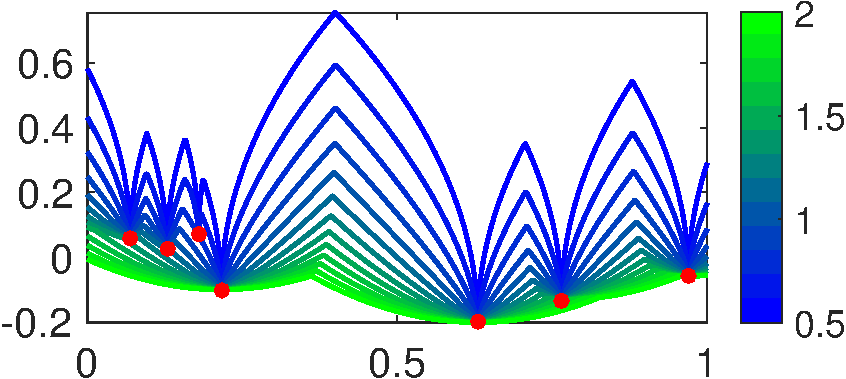
\includegraphics[width=.8\linewidth]{c-transform-1d/c-transform-p.pdf}\vspace{2mm}
%%% 2D %%%
\begin{tabular}{@{}c@{\hspace{1mm}}c@{\hspace{1mm}}c@{\hspace{1mm}}c@{}}
\MyFigCTrans{5}&
\MyFigCTrans{10}&
\MyFigCTrans{15}&
\MyFigCTrans{20}\\
$p=1/2$ & $p=1$ & $p=3/2$ & $p=2$ 
\end{tabular}
\caption{\label{fig-c-transform-discrete}
Top: examples of semidiscrete $\bar c$-transforms $\gD^{\bar \c}$ in one dimension, for ground cost $c(x,y)=|x-y|^p$ for varying $p$ (see colorbar). 
%
The red points are at locations $(y_j,-\gD_j)_j$. 
%
Bottom: examples of semidiscrete $\bar c$-transforms $\gD^{\bar \c}$ in two dimensions, for ground cost $c(x,y)=\norm{x-y}_2^p=(\sum_{i=1}^d \abs{x_i-y_i})^{p/2}$ for varying $p$. 
%
The red points are at locations $y_j \in \RR^2$, and their size is proportional to $\gD_j$. 
%
The regions delimited by bold black curves are the Laguerre cells $(\Laguerre_{j}(\gD))_j$ associated to these points $(y_j)_j$. 
}
\end{figure}

Crucially, using the discrete $\bar c$-transform in the semidiscrete problem~\eqref{eq-semi-dual-cont} yields a finite-dimensional optimization, 
\eql{\label{eq-semi-dual-discr}
	\MK_\c(\al,\be) = 
		\umax{\gD \in \RR^m}
			\Ee(\gD) \eqdef 
			\int_\X \gD^{\bar \c}(x) \d\al(x) + \sum \gD_y \b_j.
}

The Laguerre cells associated to the dual weights $\gD$
\eq{
	\Laguerre_{j}(\gD) \eqdef \enscond{x \in \X}{ \foralls j' \neq j, \c(x,y_j) - \gD_j \leq \c(x,y_{j'}) - \gD_{j'} }
}
induce a disjoint decomposition of $\X = \bigcup_j \Laguerre_{j}(\gD)$. When $\gD$ is constant, the Laguerre cells decomposition corresponds to the Voronoi diagram partition of the space. 
%
Figure~\ref{fig-c-transform-discrete}, bottom row, shows examples of Laguerre cells segmentations in two dimensions. 

This allows one to conveniently rewrite the minimized energy as
\eql{\label{eq-semi-disc-energy}
	\Ee(\gD) = \sum_{j=1}^m \int_{\Laguerre_{j}(\gD)} \pa{ c(x,y_j) - \gD_j } \d\al(x) + \dotp{\gD}{\b}.
}
The gradient of this function can be computed as follows:
\eq{
	\foralls j \in \range{m}, \quad
	\nabla\Ee(\gD)_j = - \int_{\Laguerre_{j}(\gD)} \d\al(x) + \b_j.
}
Figure~\ref{fig-semi-discr} displays iterations of a gradient descent to minimize $\Ee$.
%
Once the optimal $\gD$ is computed, then the optimal transport map $\T$ from $\al$ to $\be$ is mapping any $x \in \Laguerre_{j}(\gD)$ toward $y_j$, so it is piecewise constant. 

In the special case $\c(x,y)=\norm{x-y}^2$, the decomposition in Laguerre cells is also known as a ``power diagram.'' 
%
The cells are polyhedral and can be computed efficiently using computational geometry algorithms; see~\citep{aurenhammer1987power}. 
%
The most widely used algorithm relies on the fact that the power diagram of points in $\RR^\dim$ is equal to the projection on $\RR^\dim$ of the convex hull of the set of points $( (y_j,\norm{y_j}^2 - \gD_j) )_{j=1}^m \subset \RR^{\dim+1}$. There are numerous algorithms to compute convex hulls; for instance, that of~\citet{chan1996optimal} in two and three dimensions has complexity $O(m\log(Q))$, where $Q$ is the number of vertices of the convex hull.
%
\todoK{Maybe make a drawing of this projection.}

%\newcommand{\MyFigSemiD}[1]{\includegraphics[width=.19\linewidth]{semi-discrete/#1}}
%\begin{figure}[h!]
%\centering
%\begin{tabular}{@{}c@{\hspace{1mm}}c@{\hspace{1mm}}c@{\hspace{1mm}}c@{\hspace{1mm}}c@{}}
%\MyFigSemiD{iteration-1} &
%\MyFigSemiD{iteration-3} &
%%\MyFigSemiD{iteration-8} &
%\MyFigSemiD{iteration-9} &
%\MyFigSemiD{iteration-13} &
%\MyFigSemiD{matching} \\ 
%$\ell=1$ &
%$\ell=3$ &
%$\ell=50$ &
%$\ell=100$ &
%Matching
%\end{tabular}
%\caption{\label{fig-semi-discr}
%Iterations of the semi-discrete OT algorithm minimizing~\eqref{eq-semi-disc-energy} (here a simple gradient descent is used).
%%
%The support $(y_j)_j$ of the discrete measure $\be$ is indicated by the red points, while the continuous measure $\al$ is the uniform measure on a square. 
%%
%The blue cells display the Laguerre partition $( \Laguerre_{j}( \it{\gD} ) )_j$ where $\it{\gD}$ is the discrete dual potential computed at iteration $\ell$. 
%}
%\end{figure}

\newcommand{\MyFigSemiD}[1]{\includegraphics[width=.19\linewidth]{semidiscrete-gd/#1}}
\begin{figure}[h!]
\centering
\begin{tabular}{@{}c@{\hspace{1mm}}c@{\hspace{1mm}}c@{\hspace{1mm}}c@{\hspace{1mm}}c@{}}
\MyFigSemiD{inputs} &
\MyFigSemiD{001} &
\MyFigSemiD{020} &
\MyFigSemiD{040} &
\MyFigSemiD{100}   \\ 
$\al$ and $\be$ &
$\ell=1$ &
$\ell=20$ &
$\ell=40$ &
$\ell=100$ 
\end{tabular}
\caption{\label{fig-semi-discr}
Iterations of the semidiscrete OT algorithm minimizing~\eqref{eq-semi-disc-energy} (here a simple gradient descent is used).
%
The support $(y_j)_j$ of the discrete measure $\be$ is indicated by the colored points, while the continuous measure $\al$ is the uniform measure on a square. 
%
The colored cells display the Laguerre partition $( \Laguerre_{j}( \it{\gD} ) )_j$ where $\it{\gD}$ is the discrete dual potential computed at iteration $\ell$. 
}
\end{figure}


The initial idea of a semidiscrete solver for Monge--Amp\`ere equations was proposed by~\citet{oliker1989numerical}, and its relation to the dual variational problem was shown by~\citet{AurenhammerHA98}.
% 
A theoretical analysis and its application to the reflector problem in optics is detailed in~\citep{caffarelli1999problem}. 
%
The semidiscrete formulation was used in~\citep{carlier2010knothe} in conjunction with a continuation approach based on Knothe's transport. 
%
The recent revival of this methods in various fields is due to~\citet{Merigot11}, who proposed a quasi-Newton solver and clarified the link with concepts from computational geometry. We refer to~\citep{Levy2017review} for a recent overview. The use of a Newton solver which is applied to sampling in computer graphics is proposed in~\citep{de2012blue}; see also~\citep{levy2015numerical} for applications to 3-D volume and surface processing. 
%
An important area of application of the semidiscrete method is for the resolution of the incompressible fluid dynamic (Euler's equations) using Lagrangian methods~\citep{deGoes2015,gallouet2017lagrangian}. The semidiscrete OT solver enforces incompressibility at each iteration by imposing that the (possibly weighted) points cloud approximates a uniform distribution inside the domain.  
%
The convergence (with linear rate) of damped Newton iterations is proved in~\citep{mirebeau2015discretization} for the Monge--Amp\`ere equation and is refined in~\citep{kitagawa2016newton} for optimal transport. Semidiscrete OT finds important applications to illumination design, notably reflectors; see~\citep{merigot2017light}.

%%%%%%%%%%%%%%%%%%%%%%%%%%%%%%%%%%%%%%%%%%%%
\section{Entropic Semidiscrete Formulation}
\label{sec-semi-discr-entropy}

The dual of the entropic regularized problem between arbitrary measures~\eqref{eq-entropic-generic} is a smooth unconstrained optimization problem:
\begin{equation}\label{eq-dual-entropic-generic}
	\MK_\c^\epsilon(\al,\be) = 
	\usup{(\f,\g) \in \Cc(\X) \times \Cc(\Y)}
		 \int_\X \f\d\al + \int_\Y \g\d\be 
		- \epsilon \int_{\X \times \Y}  e^{ \frac{-c + \f \oplus \g }{\epsilon} } \d\al\d\be,
\end{equation}
where we denoted $(f\oplus g)(x,y) \eqdef f(x)+g(y)$.

Similarly to the unregularized problem~\eqref{eq-c-transform}, one can minimize explicitly with respect to either $\f$ or $\g$ in~\eqref{eq-dual-entropic-generic}, which yields a smoothed $\c$-transform
\begin{align*}
	\foralls y \in \Y, \quad
	\f^{\c,\epsilon}(y) &\eqdef - \epsilon \log\pa{ 
			\int_{\X} e^{\frac{-\c(x,y) + \f(x)}{\epsilon}} \d\al(x)
	},\\
	\foralls x \in \X, \quad
	\g^{\bar\c,\epsilon}(x) &\eqdef - \epsilon \log\pa{ 
			\int_{\Y} e^{\frac{-\c(x,y) + \g(y)}{\epsilon}} \d\be(y)
	}.
\end{align*}
In the case of a discrete measure $\be = \sum_{j=1}^m \b_j\de_{y_j}$, the problem simplifies as with~\eqref{eq-semi-dual-discr} to a finite-dimensional problem expressed as a function of the discrete dual potential $\gD \in \RR^m$, 
\eql{\label{eq-entropic-smoothed-c}
	\foralls x \in \X, \quad
	\gD^{\bar\c,\epsilon}(x) \eqdef - \epsilon \log\pa{ 
		\sum_{j=1}^m e^{\frac{-\c(x,y_j) + \gD_j}{\epsilon}} \b_j
	}.
}
One defines similarly $\fD^{\bar\c,\epsilon}$ in the case of a discrete measure $\al$.
%
Note that the rewriting~\eqref{eq-lse-dual-1} and~\eqref{eq-lse-dual-2} of Sinkhorn using the soft-min operator $\smine$ corresponds to the alternate computation of entropic smoothed $\c$-transforms,
\eql{\label{eq-sinkh-c-transf}
	\itt{\fD}_i = \gD^{\bar\c,\epsilon}(x_i) 
	\qandq
	\itt{\gD}_j = \fD^{\,\c,\epsilon}(y_j) .
}

Instead of maximizing~\eqref{eq-dual-entropic-generic}, one can thus solve the following finite-dimensional optimization problem:
\eql{\label{eq-semi-disc-energy-entropy}
	\umax{\gD \in \RR^n}
		\Ee^\epsilon(\gD) \eqdef \int_\X \gD^{\bar\c,\epsilon}(x)\d\al(x) + \dotp{\gD}{\b}.
}
Note that this optimization problem is still valid even in the unregularized case $\epsilon=0$ and in this case $\gD^{\bar\c,\epsilon=0}=\gD^{\bar\c}$ is the $\bar \c$-transform defined in~\eqref{eq-disc-c-transfo} so that~\eqref{eq-semi-disc-energy-entropy} is in fact~\eqref{eq-semi-disc-energy}.
%
The gradient of this functional reads
\eql{\label{eq-grad-semid-entrop}
	\foralls j \in \range{m}, \quad
	\nabla\Ee^\epsilon(\gD)_j = - \int_{\X} \chi_j^\epsilon(x) \d\al(x) + \b_j, 
}
where $\chi_j^\epsilon$ is a smoothed version of the indicator $\chi_j^0$ of the Laguerre cell $\Laguerre_{j}(\gD)$,
\eq{
	\chi_j^\epsilon(x) = 
	\frac{
		e^{\frac{-\c(x,y_j) + \gD_j}{\epsilon}}
	}{
		\sum_\ell e^{\frac{-\c(x,y_\ell) + \gD_\ell}{\epsilon}}
	}.
}
Note once again that this formula~\eqref{eq-grad-semid-entrop} is still valid for $\epsilon=0$.
%
Note also that the family of functions $( \chi_j^\epsilon )_j$ is a partition of unity, \ie $\sum_j \chi_j^\epsilon=1$ and $\chi_j^\epsilon \geq 0$. Figure~\ref{fig-c-transform-discrete-eps}, bottom row, illustrates this. 

%%%%%%%%%%
\begin{rem}[Second order methods and connection with logistic regression]\label{rem-second-order-smoothness}
	A crucial aspect of the smoothed semidiscrete formulation~\eqref{eq-semi-disc-energy-entropy} is that it corresponds to the minimization of a smooth function.
	%
	Indeed, as shown in~\citep{genevay2016stochastic}, the Hessian of $\Ee^\epsilon$ is upper bounded by $1/\epsilon$, so that $\nabla \Ee^\epsilon$ is $\frac{1}{\epsilon}$-Lipschitz continuous.
	%
	In fact, that problem is very closely related to a multiclass logistic regression problem (see Figure~\ref{fig-c-transform-discrete-eps} for a display of the resulting fuzzy classification boundary) and enjoys the same favorable properties (see~\citep{hosmer2013applied}), which are generalizations of self-concordance; see~\citep{bach2010self}. 
	%
	In particular, the Newton method converges quadratically, and one can use in practice quasi-Newton techniques, such as L-BFGS, as advocated in~\citep{2016-Cuturi-siims}. Note that~\citep{2016-Cuturi-siims} studies the more general barycenter problem detailed in~\S\ref{sec-bary}, but it is equivalent to this semidiscrete setting when considering only a pair of input measures. 
	%
	The use of second order schemes (Newton or L-BFGS) is also advocated in the unregularized case $\epsilon=0$ by~\citep{Merigot11,de2012blue,levy2015numerical}. In \citep[Theo. 5.1]{kitagawa2016newton}, the Hessian of $\Ee^0(\gD)$ is shown to be uniformly bounded as long as the volume of the Laguerre cells is bounded by below and $\al$ has a continuous density. \citeauthor{kitagawa2016newton} proceed by showing the linear convergence of a damped Newton algorithm with a backtracking to ensure that the Laguerre cells never vanish between two iterations. This result justifies the use of second order methods even in the unregularized case. The intuition is that, while the conditioning of the entropic regularized problem scales like $1/\epsilon$, when $\epsilon=0$, this conditioning is rather driven by $m$, the number of samples of the discrete distribution (which controls the size of the Laguerre cells).
	%
	Other methods exploiting second order schemes were also recently studied by~\citep{knight2013fast,sugiyama2017tensor,cohen2017matrix,allen2017much}.
\end{rem}
%%%%%%%%%




% G/B/D/H \fbox
\newcommand{\MyFigCTransEps}[1]{\includegraphics[width=.245\linewidth,trim=63 40 48 30,clip]{c-transform-2d/c-transform-eps#1}}
\begin{figure}[h!]
\centering
%%% 1D %%%
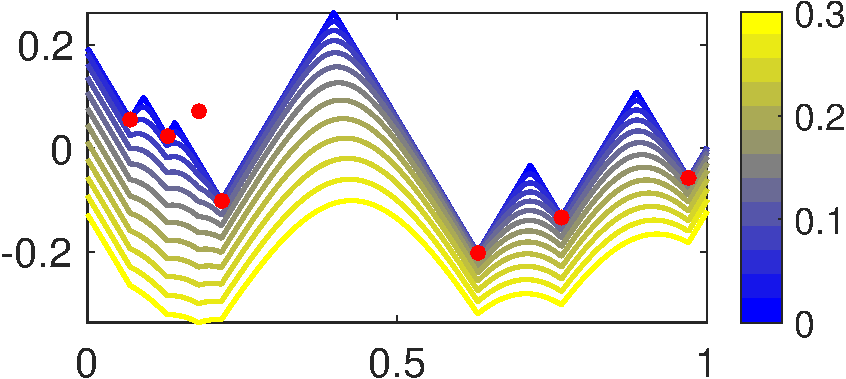
\includegraphics[width=.9\linewidth]{c-transform-1d/c-transform-eps.pdf}\vspace{2mm}
%%% 2D %%%
\begin{tabular}{@{}c@{\hspace{1mm}}c@{\hspace{1mm}}c@{\hspace{1mm}}c@{}}
\MyFigCTransEps{0}&
\MyFigCTransEps{1}&
\MyFigCTransEps{10}&
\MyFigCTransEps{30}\\
$\epsilon=0$ & $\epsilon=0.01$ & $\epsilon=0.1$ & $\epsilon=0.3$ 
\end{tabular}
\caption{\label{fig-c-transform-discrete-eps}
Top: examples of entropic semidiscrete $\bar c$-transforms $\gD^{\bar \c,\epsilon}$ in one dimension, for ground cost $c(x,y)=|x-y|$ for varying $\epsilon$ (see colorbar). 
%
The red points are at locations $(y_j,-\gD_j)_j$. 
%
Bottom: examples of entropic semidiscrete $\bar c$-transforms $\gD^{\bar \c,\epsilon}$ in two dimensions, for ground cost $c(x,y)=\norm{x-y}_2$ for varying $\epsilon$. The black curves are the level sets of the function $\gD^{\bar \c,\epsilon}$, while the colors indicate the smoothed indicator function of the Laguerre cells $\chi_j^\epsilon$.
%
The red points are at locations $y_j \in \RR^2$, and their size is proportional to $\gD_j$. 
}
\end{figure}



%%%%%%%%%%
\begin{rem}[Legendre transforms of OT cost functions] 
	As stated in Proposition~\ref{prop-convexity-dual}, $\MKD_\C^\epsilon(\a,\b)$ is a convex function of $(\a,\b)$ (which is also true in the unregularized case $\epsilon=0$). 
	%
	It is thus possible to compute its Legendre--Fenchel transform, which is defined in~\eqref{eq-legendre}.
	%
	Denoting $F_\a(\b) = \MKD_\C^\epsilon(\a,\b)$, one has, for a fixed $\a$, following~\citet{2016-Cuturi-siims}:
	\eq{
		F_\a^*(\gD) =  - \epsilon H(\a) + \sum_i \a_i \gD^{\bar\c,\epsilon}(x_i).
	}
	Here $\gD^{\bar\c,\epsilon}$ is the entropic-smoothed $c$-transform introduced in~\eqref{eq-entropic-smoothed-c}.
	%
	In the unregularized case $\epsilon=0$, and for generic measures,~\citet{Carlier-NumericsBarycenters} show, 	
	denoting $\Ff_\al(\be) \eqdef \MK_\c(\al,\be)$,
	\eq{
		\foralls \g \in \Cc(\Y), \quad
		\Ff_\al^*(\g) = \int_\X \g^{\bar\c}(x)  \d\al(x), 		
	}
	where the $\bar c$-transform $\g^{\bar c} \in \Cc(\X)$ of $\g$ is defined in~\S\ref{s-c-transform}.
%	denoting $\Ff_\be(\al) \eqdef \MK_\c(\al,\be)$,
%	\eq{
%		\foralls \f \in \Cc(\X), \quad
%		\Ff_\be^*(\f) = \int_\Y \f^{\c}(y)  \d\be(y), 		
%	}
%	where the $c$-transform $\f^c \in \Cc(\Y)$ of $\f$ was defined in~\S\ref{s-c-transform}.
	%
	Note that here, since $\Mm(\X)$ is in duality with $\Cc(\X)$, the Legendre transform is a function of continuous functions.
	%
	Denoting now $G(\a,\b) \eqdef \MKD_\C^\epsilon(\a,\b)$, one can derive as in~\citep{2016-Cuturi-siims,cuturi2018semidual} the Legendre transform for both arguments,
	\eq{
		\foralls (\fD,\gD) \in \RR^n \times \RR^m, \quad
		G^*(\fD,\gD) = - \epsilon \log \sum_{i,j} e^{ \frac{-\C_{i,j}+\fD_i+\gD_j}{\epsilon} },
	} 
	which can be seen as a smoothed version of the Legendre transform of $\Gg(\al,\be) \eqdef \MK_\c(\al,\be)$,
	\eq{
		\foralls (\f,\g) \in \Cc(\X) \times \Cc(\Y), \quad
		\Gg^*(\f,\g) = \uinf{(x,y) \in \X \times \Y} \c(x,y)-\f(x)-\g(y).	
	}
\end{rem}
%%%%%%%%%%



%%%%%%%%%%%%%%%%%%%%%%%%%%%%%%%%%%%%%%%%%%%%
\section{Stochastic Optimization Methods}
\label{sec-sgd}

The semidiscrete formulation~\eqref{eq-semi-disc-energy} and its smoothed version~\eqref{eq-semi-disc-energy-entropy} are appealing because the energies to be minimized are written as an expectation with respect to the probability distribution $\al$,
\eq{
	\Ee^\epsilon(\gD) = \int_\X E^\epsilon(\gD,x) \d\al(x) = \EE_X(  E^\epsilon(\gD,X) )
}
\eq{
	\qwhereq
	 E^\epsilon(\gD,x) \eqdef 
	\gD^{\bar\c,\epsilon}(x) - \dotp{\gD}{\b},
}
and $X$ denotes a random vector distributed on $\X$ according to $\al$.
%
Note that the gradient of each of the involved functional reads
\eq{
	\nabla_{\gD} E^\epsilon(x,\gD) = (  \chi_j^\epsilon(x) - \b_j )_{j=1}^m \in \RR^m.
}
%
One can thus use stochastic optimization methods to perform the maximization, as proposed in~\citet{genevay2016stochastic}.
%
This allows us to obtain provably convergent algorithms without the need to resort to an arbitrary discretization of $\al$ (either approximating $\al$ using sums of Diracs or using quadrature formula for the integrals).
%
The measure $\al$ is used as a black box from which one can draw independent samples, which is a natural computational setup for many high-dimensional applications in statistics and machine learning. 
%
This class of methods has been generalized to the computation of Wasserstein barycenters (as described in \S\ref{sec-bary}) in~\citep{staib2017parallel}.

%%%%
\paragraph{Stochastic gradient descent.}

Initializing $\gD^{(0)} = \zeros_{P}$, the stochastic gradient descent algorithm (SGD; used here as a maximization method) draws at step $\ell$ a point $x_\ell \in \X$ according to distribution $\al$ (independently from all past and future samples $(x_\ell)_\ell$) to form the update
\eql{\label{eq-sgd}
	\itt{\gD} \eqdef \it{\gD} + \tau_\ell  \nabla_{\gD} E^\epsilon(\it{\gD},x_\ell).
} 
The step size $\tau_\ell$ should decay fast enough to zero in order to ensure that the ``noise'' created by using  $\nabla_{\gD} E^\epsilon(x_\ell,\gD)$ as a proxy for the true gradient $\nabla \Ee^\epsilon(\gD)$ is canceled in the limit. 
%
A typical choice of schedule is 
\eql{\label{eq-step-size-sgd} 
	\tau_\ell \eqdef \frac{\tau_0}{1 + \ell/\ell_0}, 
}
where $\ell_0$ indicates roughly the number of iterations serving as a warmup phase.
%
One can prove the convergence result
\eq{ 
	\Ee^\epsilon(\gD^\star) - \EE( \Ee^\epsilon(\it{\gD}) ) = O\pa{ \frac{1}{\sqrt{\ell}} }, 
}
where $\gD^\star$ is a solution of~\eqref{eq-semi-disc-energy-entropy} and where $\EE$ indicates an expectation with respect to the i.i.d. sampling of $(x_\ell)_\ell$ performed at each iteration.
%
Figure~\ref{fig-semi-discrete-sgd} shows the evolution of the algorithm on a simple 2-D example, where $\al$ is the uniform distribution on $[0,1]^2$. 


\begin{figure}[h!]
\centering
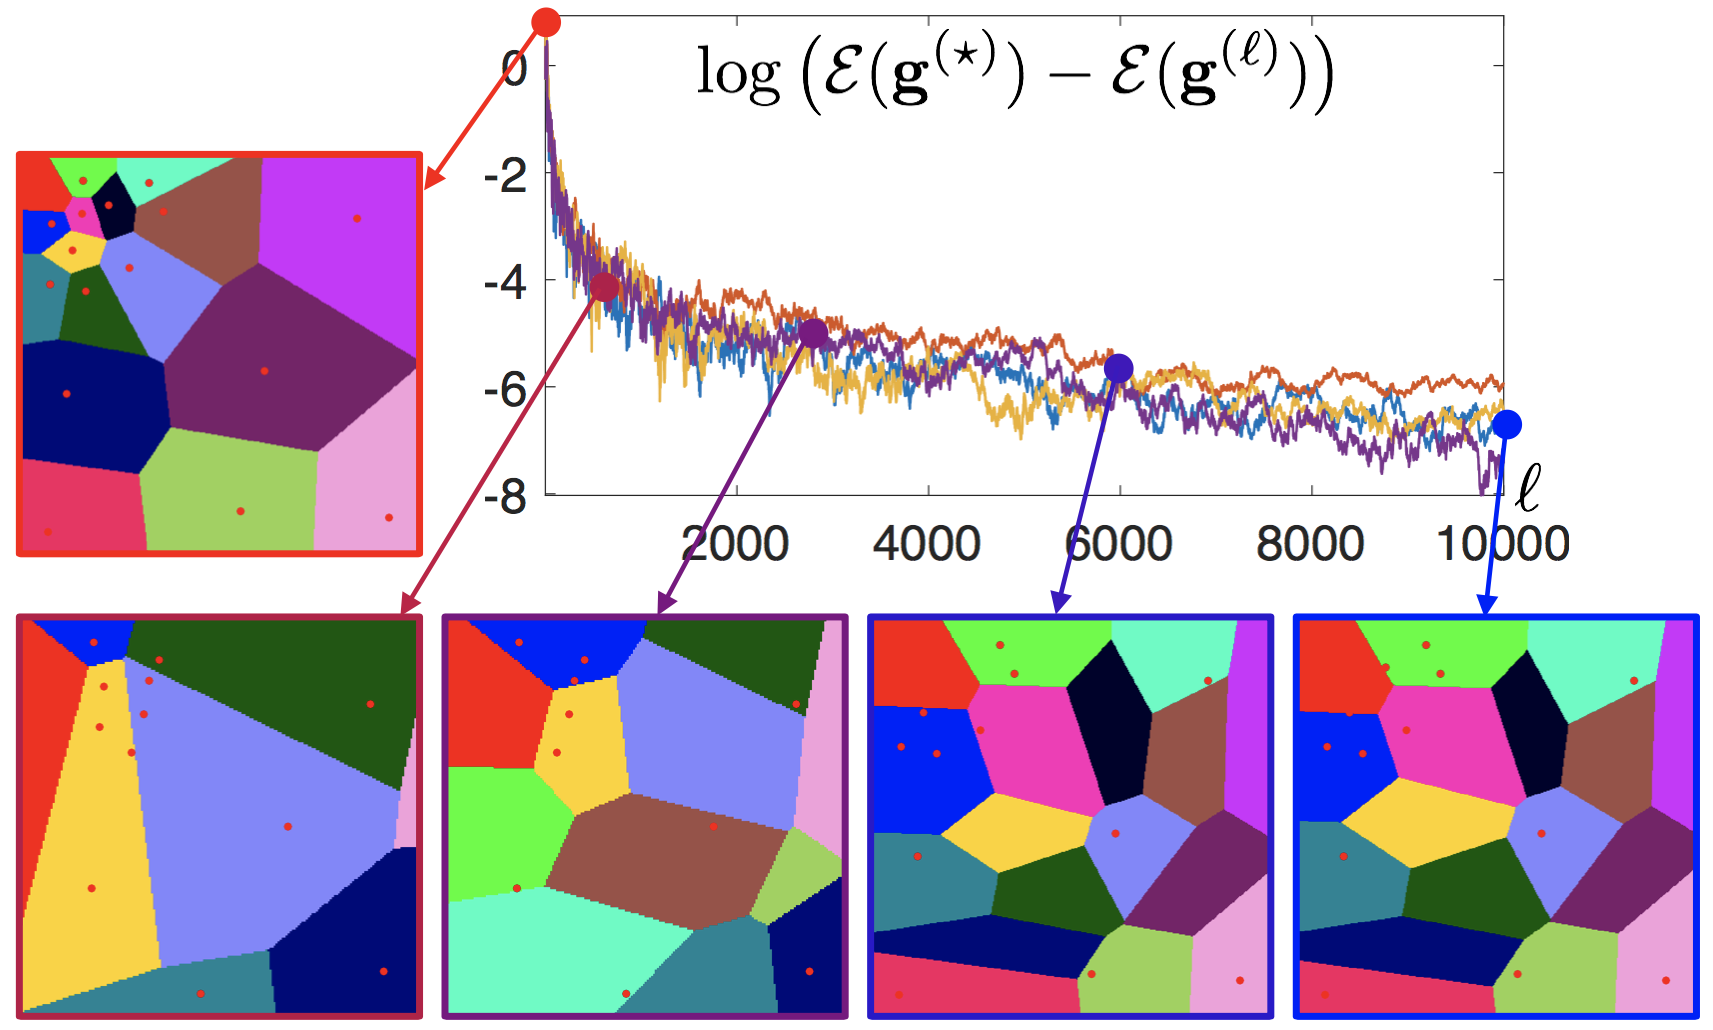
\includegraphics[width=.95\linewidth]{semi-discrete-sgd/semi-discrete-sgd}
\caption{\label{fig-semi-discrete-sgd}
Evolution of the energy $\Ee^\epsilon(\it{\gD})$, for $\epsilon=0$ (no regularization) during the SGD iterations~\eqref{eq-sgd}. Each colored curve shows a different randomized run.
%
The images display the evolution of the Laguerre cells $( \Laguerre_{j}(\it{\gD}) )_j$ through the iterations. 
}
\end{figure}

%%%%
\paragraph{Stochastic gradient descent with averaging.}

SGD is slow because of the fast decay of
the stepsize $\tau_\ell$ toward zero.
%
To improve the convergence speed, it is possible to average the past
iterates, which is equivalent to running a ``classical'' SGD on auxiliary variables $(\it{\tilde\gD})_\ell$
\eq{ 	
	\itt{\tilde\gD} \eqdef  \it{\tilde\gD} + \tau_\ell \nabla_{\gD} E^\epsilon(\it{\tilde\gD},x_\ell),
}
where $x_\ell$ is drawn according to $\al$ (and all the $(x_\ell)_\ell$ are independent)
and output as estimated weight vector the average
\eq{ 
	\it{\gD} \eqdef \frac{1}{\ell} \sum_{k=1}^\ell  \tilde\gD^{(k)}. 
}
This defines the stochastic gradient descent with averaging (SGA)
algorithm.
%
Note that it is possible to avoid explicitly storing all the iterates by simply
updating a running average as follows:
\eq{ 
	\itt{\gD} = \frac{1}{\ell+1}  \itt{\tilde\gD} +  \frac{\ell}{\ell+1} \it{\gD}.
}
%
In this case, a typical choice of decay is rather of the form 
\eq{ 
	\tau_\ell \eqdef \frac{\tau_0}{1 + \sqrt{\ell/\ell_0}}. 
}
Notice that the step size now goes much slower to 0 than for~\eqref{eq-step-size-sgd}, at rate $\ell^{-1/2}$.
%
\citet{bach2014adaptivity} proves that SGA leads to a faster convergence (the constants involved are smaller) than SGD, since in contrast to SGD, SGA is adaptive to the local strong convexity (or concavity for maximization problems) of the functional.




%%%%%%%%%%
\begin{rem}[Continuous-continuous problems]\label{rem-sgd-cont-cont}
When neither $\al$ nor $\be$ is a discrete measure, one cannot resort to semidiscrete strategies involving finite-dimensional dual variables, such as that given in Problem~\eqref{eq-semi-dual-discr}. The only option is to use stochastic optimization methods on the dual problem~\eqref{eq-dual-entropic}, as proposed in~\citep{genevay2016stochastic}. A suitable regularization of that problem is crucial, for instance by setting an entropic regularization strength $\epsilon>0$, to obtain an unconstrained problem that can be solved by stochastic descent schemes.
%
A possible approach to revisit Problem~\eqref{eq-dual-entropic} is to restrict that infinite-dimensional optimization problem over a space of continuous functions to a much smaller subset, such as that spanned by multilayer neural networks~\citep{seguy2018large}. This approach leads to nonconvex finite-dimensional optimization problems with no approximation guarantees, but this can provide an effective way to compute a proxy for the Wasserstein distance in high-dimensional scenarios.
%
Another solution is to use nonparametric families, which is equivalent to considering some sort of progressive refinement, as that proposed by~\citet{genevay2016stochastic} using reproducing kernel Hilbert spaces, whose dimension is proportional to the number of iterations of the SGD algorithm. 
\end{rem}
%%%%%%%%%%
